\section{问题四：未知朝向源的覆盖与联合巡回}
\subsection{定向盲区的覆盖证书}
未知朝向意味着接收条件除距离外还要求检测点位于源发射方向的闭半平面内。本轮采用 \texttt{ring25} 同心环三角剖分：外环 16 点位于半径 $1800/\cos(\pi/16)+1\,\mathrm m$ 的正十六边形，内环 8 点位于半径 $997\,\mathrm m$ 的正八边形，再补入原点，共 25 个站点。每个 $45^\circ$ 扇区拆成三个三角形，内环区域拆成八个三角形；代码检查每个单元的最大边长不超过 $1000\,\mathrm m$，外环切线距离覆盖 $1800\,\mathrm m$ 圆盘。

设发射方向单位向量为 $d$。若某个覆盖三角形的三个顶点均满足 $d\cdot(p_j-g)<0$，则对包含 $g$ 的凸组合加权会得到 $d\cdot(g-g)<0$，矛盾。因此至少一个顶点满足闭半平面条件。该证明同时覆盖边界点、向外发射方向和源位于网格顶点的情形；外环额外留出的 1 m 只用于抵抗边界浮点舍入。

从几何上看，外环半径取 $r_o=1800/\cos(\pi/16)+1\,\mathrm m$，即在外接半径基础上增加 $1\,\mathrm m$，对应切向余量约 $0.981\,\mathrm m$；内环半径取 $r_i=997\,\mathrm m$，使中心三角形和外侧三角形的最长边均处于 1000 m 接收半径以内。程序对 32 个三角形逐一计算三条边长，并用随机圆盘点与等角圆周点做包含性采样。该数值检查是对解析证书的独立实现核对，不能替代解析证明，也不把抽样通过写成对连续域的额外定理。

环形站点和访问编号见图~\ref{fig:q4-coverage}；图中的三角形是覆盖证书单元，折线才是机器狗的站点访问路线，两者用途不同。

\begin{figure}[H]\centering
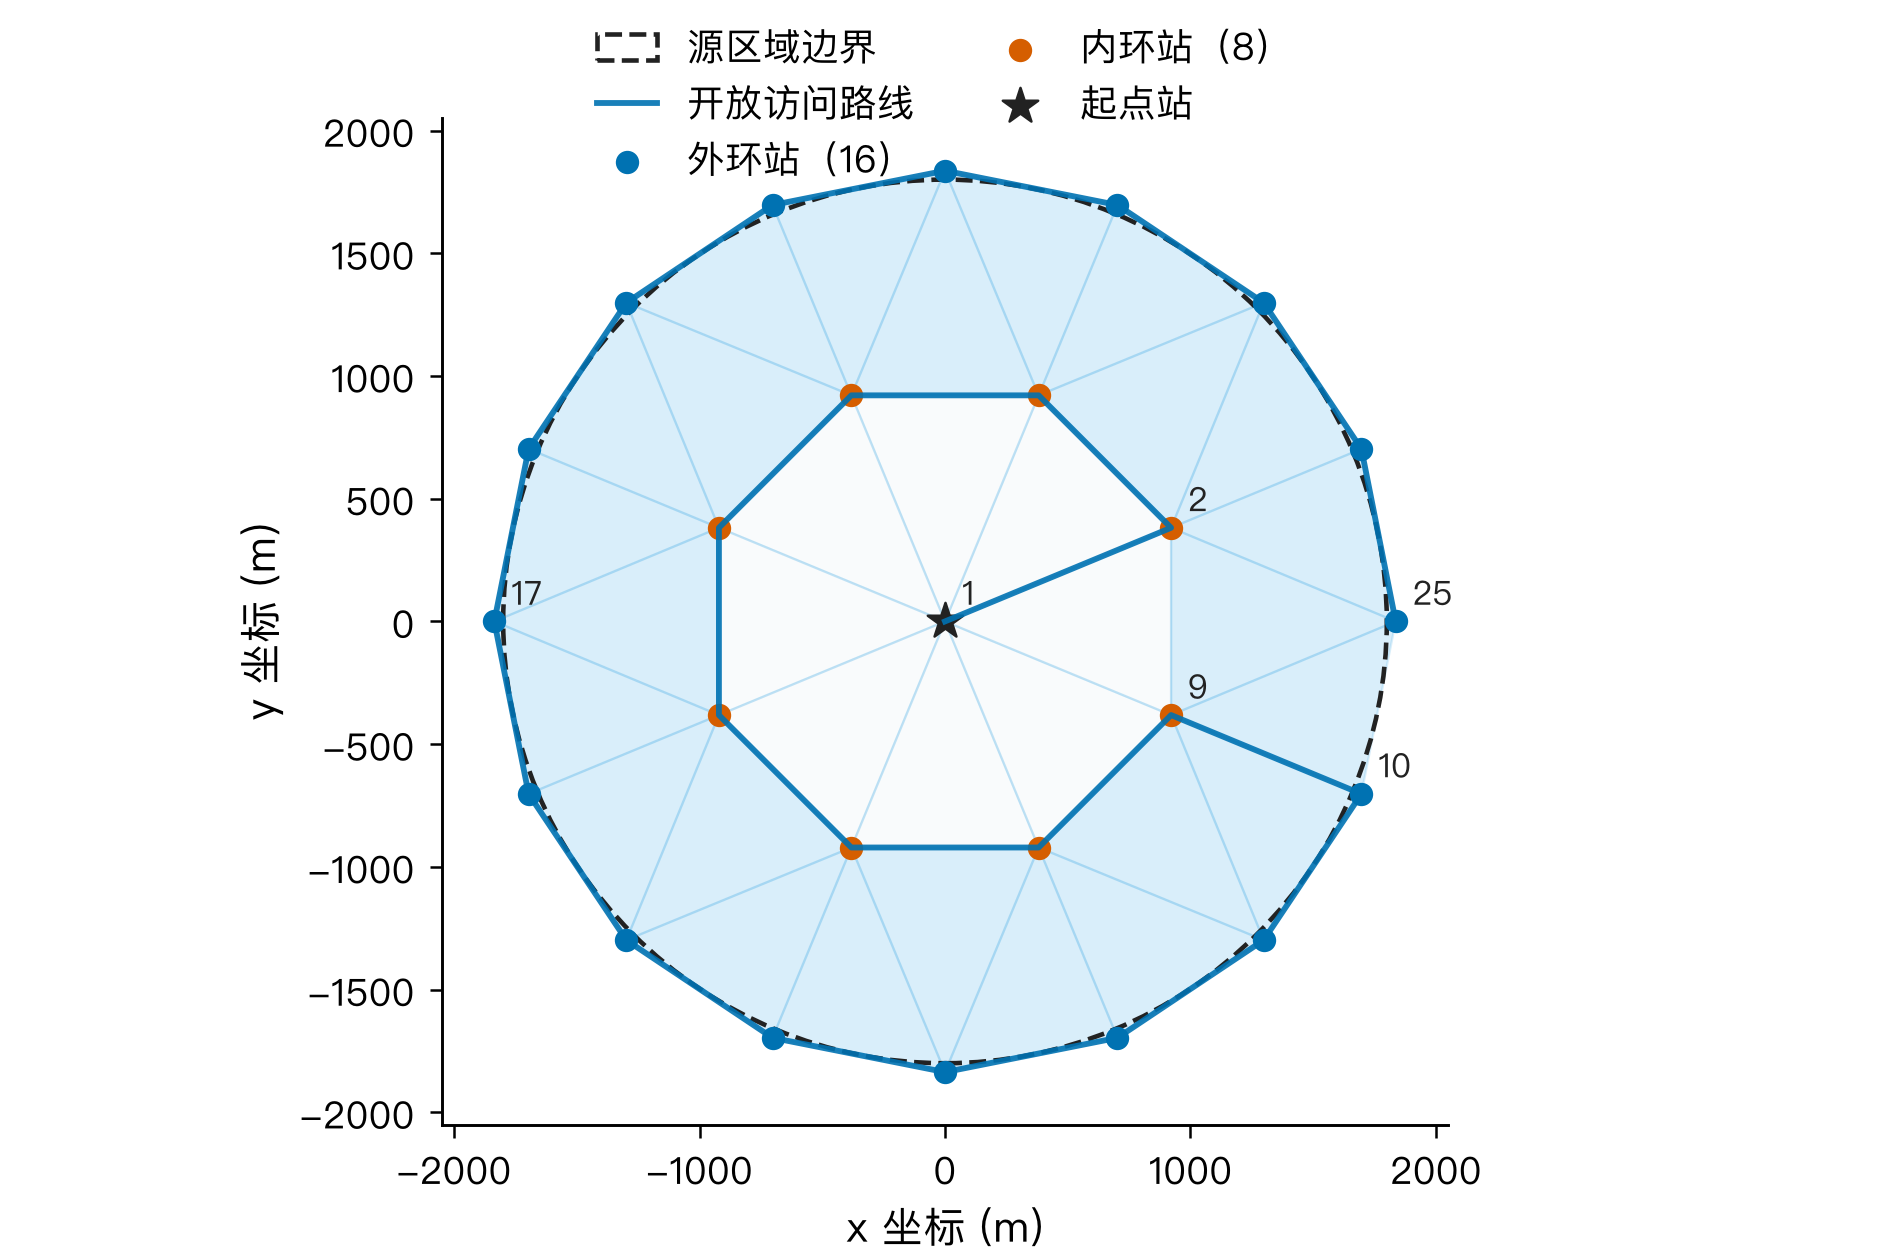
\includegraphics[width=0.82\linewidth]{figures/process_q4_coverage.png}
\caption{问题四的 25 站同心环三角覆盖与开放访问路线}\label{fig:q4-coverage}
\source{ring25_cover 的确定性构造；32 个覆盖单元，图中编号为访问顺序。}
\end{figure}

将站点集合记为 $P=\{p_0,\ldots,p_{n-1}\}$，开放访问路线 $\pi$ 的几何长度为
\begin{equation}
L_{\rm station}(\pi)=\|p_0-p_{\pi_1}\|+\sum_{i=2}^{n-1}\|p_{\pi_i}-p_{\pi_{i-1}}\|.
\end{equation}
当前实现先用最近邻生成可行顺序，再用 2-opt 反转子段；它只优化覆盖站之间的开放路径，不改变覆盖单元或清除判据。由同一段代码直接复核，25 站环形路线的站点长度为 $17{,}924.88\,\mathrm m$，26 站三角路线为 $24{,}078.75\,\mathrm m$，具体数值见表~\ref{tab:q4-route-length}。该长度不包含逐频道测量和末端目标清除的移动。

\begin{table}[H]\centering\small
\caption{覆盖站开放路线的几何长度核验}\label{tab:q4-route-length}
\begin{tabular}{lrrr}
\toprule
覆盖构造 & 站点数 & $L_{\rm station}$ (m) & 相对 26 站三角 \\
\midrule
26 站三角 & 26 & 24078.75 & 基线 \\
25 站环形 & 25 & 17924.88 & -25.56\% \\
\bottomrule
\end{tabular}
\source{src/cumcm\_b/policy.py 的 q4\_station\_route；确定性几何计算。}
\end{table}

\subsection{联合巡回策略}
覆盖阶段按固定开路径访问 25 个站点，对未知频道逐站扫描；对已有方向频道只保留最多三个当前最小包围圆半径最大的补充测向，默认不在巡回中触发光学方格。覆盖结束后，将所有已发现频道的当前包围圆圆心作为目标点，采用最近邻初始化、开放路径 2-opt 改善访问顺序，逐目标执行安全清除或有限兜底。这样的“覆盖单元—路线—末端处理”分层与公开覆盖规划库的模块化思路一致\cite{fields2cover,opennav,coverage}；有限测量名额按当前可能区域半径排序，优先处理不确定性最大的频道，滚动 q10 信息目标则在末端定位阶段执行。覆盖引导图、有限视界收益评估以及信息路径规划中的节点奖励思想分别可见 CAP、adaptive coverage、AIPP 与 SISL 的公开工作\cite{cap,adaptivecoverage,aipp,sisl}；本文只借鉴其分层与收益排序思想，清除安全仍由闭集几何证书决定。该分阶段设计还来自官方演练日志：同一未收敛频道在多个站点重复清除会产生大量无效请求。

联合目标可以写成词典序问题：首先要求所有覆盖站访问完毕且 $c_k=1$ 对所有已发现频道成立；在可行解集合内，再最小化 $T$。覆盖阶段的固定路线使几何证书与移动路线可独立复核，末端阶段的 2-opt 只改变目标访问顺序，不改变每个频道的 $R^*$ 判据。若当前目标仍未满足清除证书，算法最多进行规定次数的主动测向，随后调用与可能区域相交的光学方格；因此路线优化不会以牺牲清除安全性为代价。

图~\ref{fig:q4-route} 是两阶段策略的抽象流程，图~\ref{fig:q4-trajectory} 则把同一思想映射到过程日志中的实际动作和虚拟时间。

\begin{figure}[H]\centering
\begin{tikzpicture}[x=1cm,y=1cm]
\draw[thick,rounded corners] (-3,-1.9) rectangle (3.2,2.0);\draw[step=0.9,gray!40] (-2.8,-1.7) grid (3,1.8);
\draw[very thick,blue,->] (-2.4,-1.3)--(-1.2,0.8)--(0.0,-1.2)--(1.1,1.3)--(2.6,-0.8);
\foreach \p in {(-2.4,-1.3),(-1.2,0.8),(0,-1.2),(1.1,1.3),(2.6,-0.8)}{\fill \p circle (2pt);}
\node at (0,-2.35) {覆盖阶段收集信息，末端阶段清除目标};
\end{tikzpicture}
\caption{问题四两阶段联合巡回示意}\label{fig:q4-route}
\source{路径结构示意；真实站点坐标由程序生成。}
\end{figure}

\begin{figure}[H]\centering
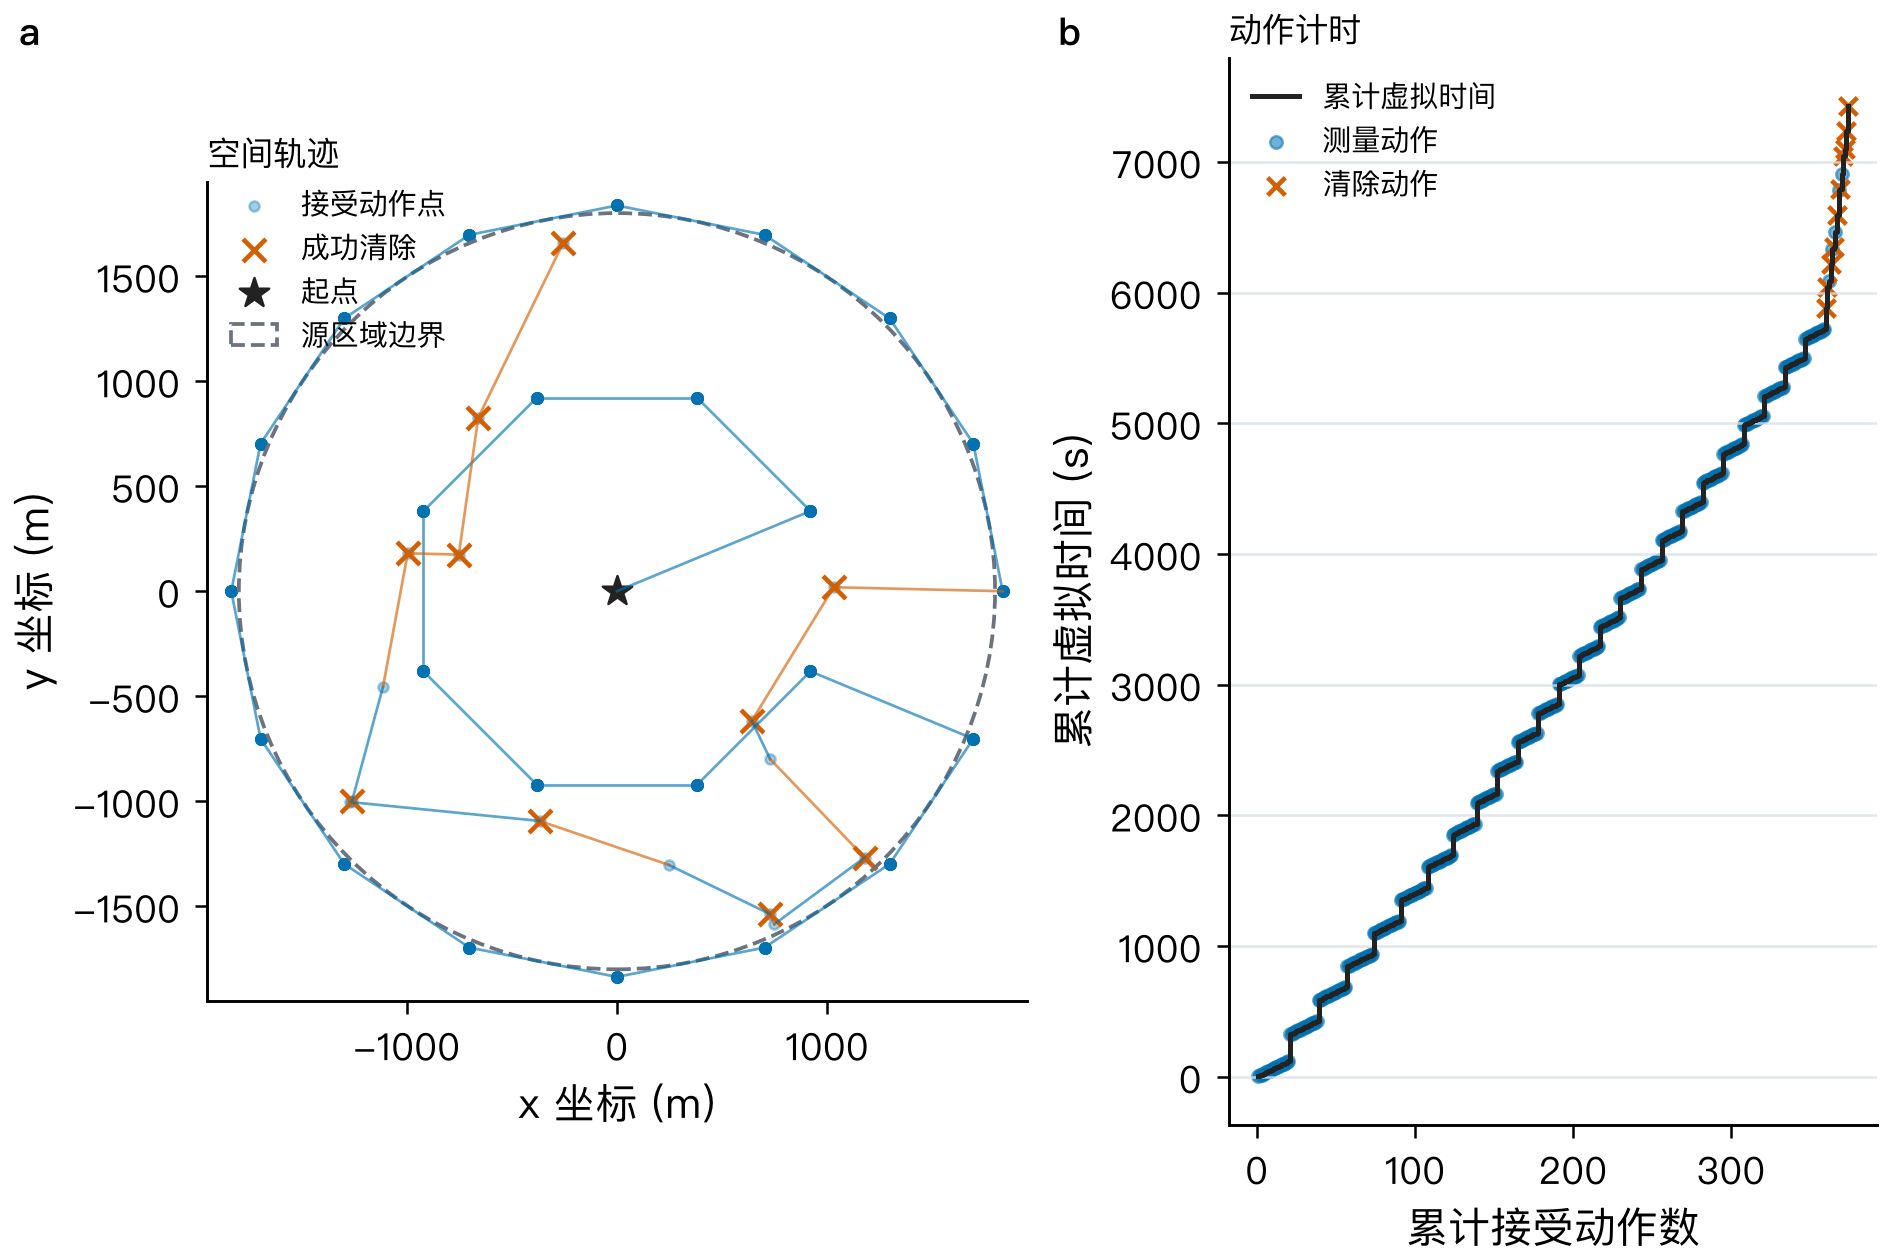
\includegraphics[width=0.98\linewidth]{figures/process_q4_trajectory.png}
\caption{问题四过程记录中的空间轨迹与累计虚拟时间}\label{fig:q4-trajectory}
\source{results/synthetic/q4_current_trace.json；q4\_joint，ring25，种子 20260911，本地合成过程记录。}
\end{figure}
